\documentclass{book}

\usepackage{amsmath}
\usepackage{geometry}
\usepackage{graphicx}

\title{A Tourists Guide to the Radio Frequency Spectrum}
\author{Delta Eight Zeta}
\graphicspath{{./images/}}



\begin{document}
    \maketitle
    \tableofcontents


    \chapter{Introduction}
    \section{What is the Radio Frequency Spectrum?}
        The Radio Frequency Spectrum is a spectrum from 20KHz to 300GHz where we measure the oscillation in waves to receive a signal whether it be a voice or data.
        Radio waves are a type of electromagnetic radiation with wavelengths in the electromagnetic spectrum longer than infrared light. 
        However RF waves very a lot in their propagation characteristics, IE shortwave radio bounces off the ionosphere and can be heard cross continental,
        meanwhile VHF and UHF are line of sight and can only be heard within a few miles.
        To clarify VHF is 30MHz to 300MHz and UHF is 300MHz to 3GHz. A good rule of thumb is that lower frequencies will get you a farther range at a cost
        of bandwidth and size of those antenna. You may be told to get hundreds of feet of wire for a shortwave antenna but only some inches for a VHF antenna,
        UHF is even shorter antenna where you need reflectors and etc.
    \section{What is the Radio Frequency Spectrum used for?}
        The RF spectrum is used for A LOT of things, from your TV, Phone, Radio, WiFi, Bluetooth, GPS, and even your Microwave.
        Whether you are an average person or a radio enthusiast, you use the RF spectrum everyday regardless. Unless if you are a 
        hermit living in the woods \ldots
        \\
        The Goal of this book will be to introduce you to the RF spectrum, antenna, gear, and etc.
        Then based on the FCC rules and regulations, I will show you some things you may do on different frequencies.
        I will also show you some things you may do on different frequencies that are not FCC approved. AT YOUR OWN RISK.
    \section{What does the RF Spectrum actually look like?}
    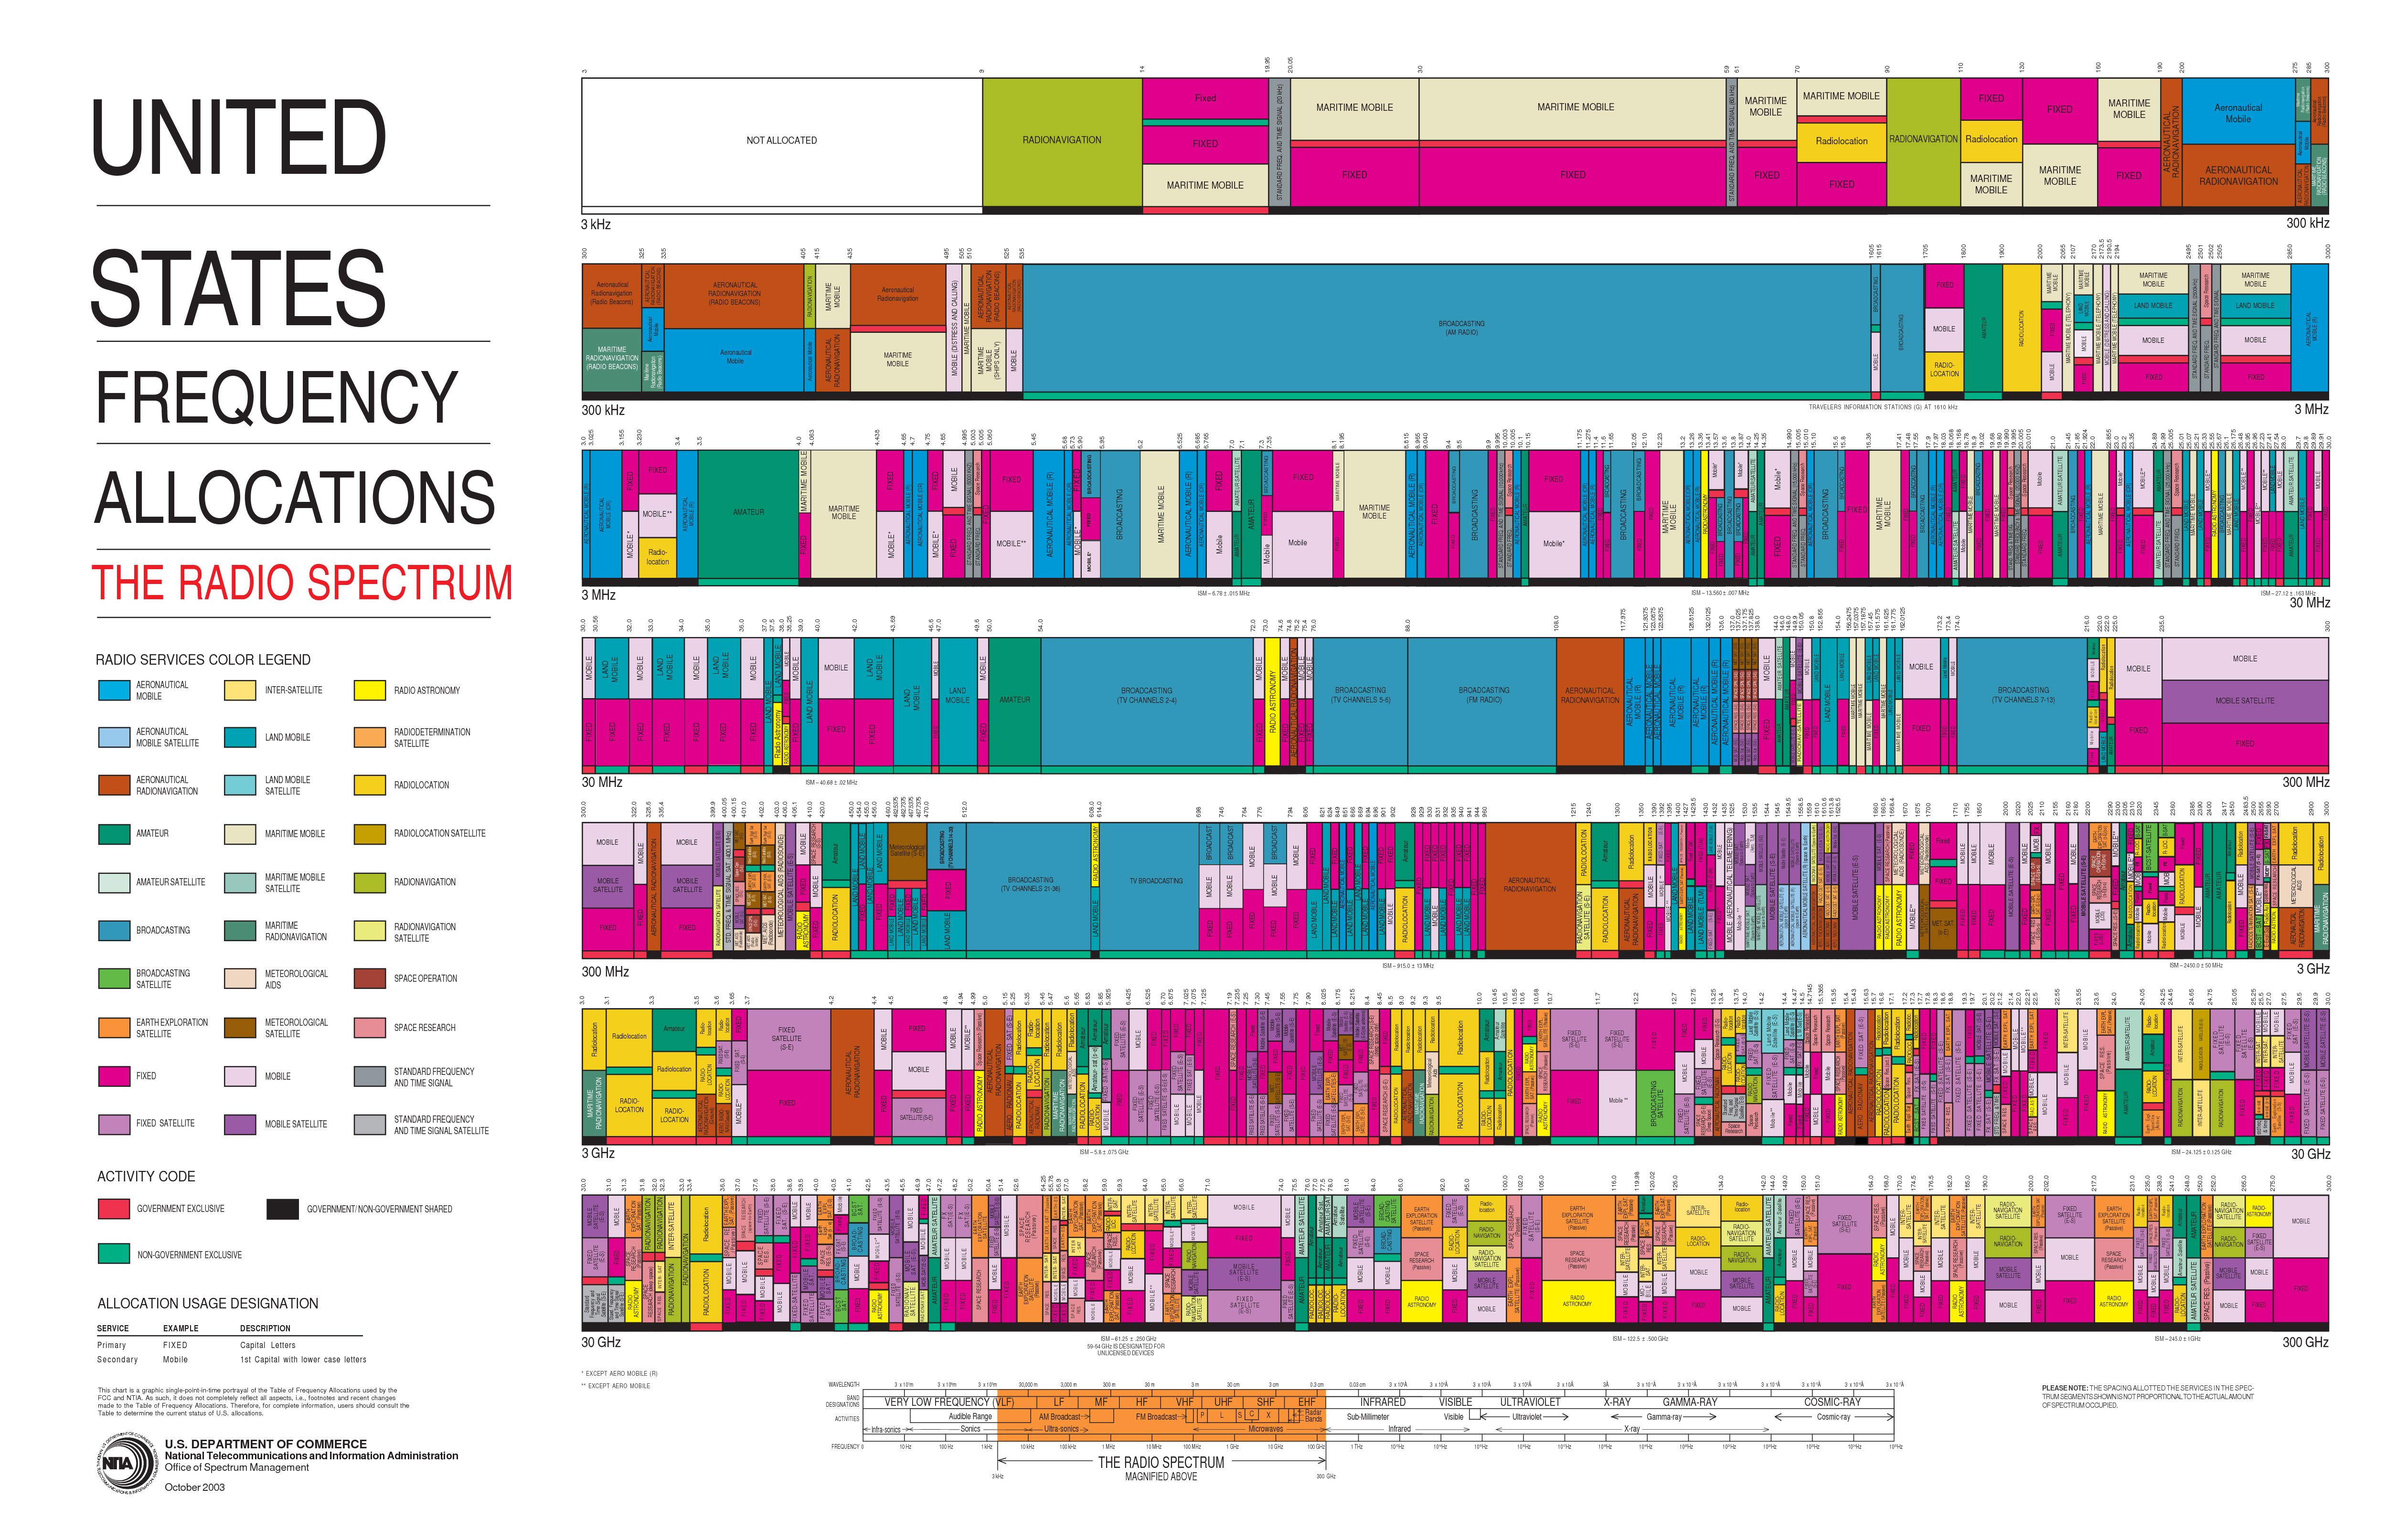
\includegraphics[width=\textwidth]{RF_Spectrum.jpg}
        Well, thats the spectrum, I have a lot to go over\ldots Its okay though.
        One step at a time and remember, a lot is repeated.

    \chapter{Radio Services and Their Uses}
    \section{Aeronautical Mobile}
        Aeronautical Mobile services are used for communication between aircraft and ground stations, or between aircraft.
        This is a protected service per-say, I would highly advise against transmitting in these frequencies 
        as they are used for emergency communications and etc.
    \section{Aeronautical Mobile Satellite}
        Aeronautical Mobile Satellite services are similar to Aeronautical Mobile however they use, guess it, Satellites.
    \section{Aeronautical Radionavigation}
        Aeronautical Radionavigation is to help navigate in the air using interferometry and etc to determain position reletive 
        to beacons. Don't transmit here.
    \section{Amateur}
        Amateur radio is a hobby where you can talk to people locally and far away with your radio.
        If you are liscensed, Transmit! There are lovely people here that would love
        to talk and have a good time. If you aren't liscensed, you can still listen in of course!
    \section{Amateur Satellite}
        Amateur Satellite is the same as Amateur however you are using Satellites to communicate. The AMSAT project is absolutely amazing and worth checking out!
    \section{Broadcasting}
        This is where your car radio is typically tuned to, high power stations that broadcast frequency and amplitude modulated signals (we will mention modulation later).
        Its that high power allowance that makes such a big difference allowing decent range and quality. I wouldn't reccomend you broadcast over these ranges unliscensed however, you might just 
        be drowned out by the stations anyways. 
    \section{Broadcasting Satellite}
        Broadcasting Satellite is the same as Broadcasting however you are using Satellites to carry signal. Often these signals are Circulary polarized and will have spiral or any Circulary polarized antenna
        this helps to have a stable quality. SiriusXM is a well known example of this.
    \section{Earth Exploration Satellite}


\end{document}